\documentclass{article}
% \usepackage{xeCJK}
\usepackage{amsmath}
\usepackage{amssymb}
\usepackage{mathrsfs}
\usepackage{xcolor}
\usepackage{bm}
\usepackage{hyperref}
\usepackage{graphicx}
\usepackage{subcaption}
\usepackage{float}
\usepackage{multicol}
\usepackage{pdfpages}
\usepackage[ruled,linesnumbered]{algorithm2e}

\bibliographystyle{plain}
\setlength{\parindent}{2em}
\usepackage{geometry}
\geometry{a4paper, left=2.54cm, right=2.54cm, top=3.18cm, bottom=3.18cm}

% 设置文章行距
% \renewcommand{\baselinestretch}{1.5}

% define reference format
\hypersetup{
    colorlinks=true,
    linkcolor=blue,
    urlcolor=blue,
    citecolor=blue,
    linkbordercolor=white
}

\title{\textbf{Hyperuniformity in Chemotactic Active Matter}}
\author{Yichen Lu}

\begin{document}

\maketitle

\tableofcontents

\section{Models}

\subsection{Particle-based model}
\begin{subequations}
    \begin{align}
        &\frac{\mathrm{d}}{\mathrm{d}t}\mathbf{r}_i\left( t \right) =\alpha \nabla c\left( \mathbf{r}_i\left( t \right) ,t \right) +\sqrt{2D}\boldsymbol{\xi }\left( t \right) \;,\\
        &\frac{\partial}{\partial t} c \left( \mathbf{r},t \right) =D_c\nabla ^2c\left( \mathbf{r},t \right) +\mu c\left( \mathbf{r},t \right) +k\sum_{j=1}^{N}{\delta \left( \mathbf{r}-\mathbf{r}_i\left( t \right) \right)}\;,
    \end{align}
\end{subequations}
for $i=1,2,\cdots,N$. Here, $\mathbf{r}_i$ is the position of the $i$-th particle, $c$ is the concentration field of the chemoattractant, $\alpha$ is the chemotactic sensitivity. If $\alpha > 0$, the particles are attracted to higher concentrations of the chemoattractant (chemoattraction/positive chemotaxis), while if $\alpha < 0$, the particles are repelled by higher concentrations of the chemoattractant (chemorepulsion/negative chemotaxis).
$D$ is the diffusion coefficient of the particles, $\boldsymbol{\xi }$ is a Gaussian white noise with zero mean and unit variance, $D_c$ is the diffusion coefficient of the chemoattractant, $\mu$ is the decay ($\mu < 0$) or growth ($\mu > 0$) rate of the chemoattractant, and $k$ is the production ($k > 0$) or consumption rate ($k < 0$) of the chemoattractant by the particles.

For simplicity, we assume that particles are point-like and move in a two-dimensional $L \times L$ square domain with periodic boundary conditions. The initial positions of the particles can be randomly distributed, and the initial concentration field can be set to a small random perturbation around a uniform background concentration $c_0$.

To reduce the parameter space, we can non-dimensionalize the equations by introducing $x_0 = L$, $t_0 = 1/k$ and $c_0$ as characteristic scales of length, time and concentration. The resulting dimensionless parameters are $\tilde{\alpha} = \frac{\alpha c_0}{L^2k}$, $\tilde{D} = \frac{D}{L^2k}$, $\tilde{D}_c = \frac{D_c}{L^2k}$, and $\tilde{\mu} = \frac{\mu}{k}$. We can omit the tildes and work with the dimensionless equations:
\begin{subequations}
    \begin{align}
        &\frac{\mathrm{d}}{\mathrm{d}t}\mathbf{r}_i\left( t \right) =\alpha \nabla c\left( \mathbf{r}_i\left( t \right) ,t \right) +\sqrt{2D}\boldsymbol{\xi }\left( t \right) \;,\\
        &\frac{\partial}{\partial t} c \left( \mathbf{r},t \right) =D_c\nabla ^2c\left( \mathbf{r},t \right) +\mu c\left( \mathbf{r},t \right) +\sum_{j=1}^{N}{\delta \left( \mathbf{r}-\mathbf{r}_i\left( t \right) \right)}\;.\label{eq:dimensionlessCplus}
    \end{align}
\end{subequations}
Note that the above equations mathematically implies the assumption of $k>0$. If $k<0$, the non-dimensionalization would be different, and the Eq.~\eqref{eq:dimensionlessCplus} would have a negative sign in front of the summation term:
\begin{equation}
    \frac{\partial}{\partial t} c\left( \mathbf{r},t \right) =D_c\nabla ^2c\left( \mathbf{r},t \right) +\mu c\left( \mathbf{r},t \right) -\sum_{j=1}^{N}{\delta \left( \mathbf{r}-\mathbf{r}_i\left( t \right) \right)}\;.
\end{equation}
In the following, we will focus on the case of $k<0$ (chemorepulsion/negative chemotaxis), which is more relevant to the emergence of hyperuniformity.

\subsection{Continuum model}
It is convenient to describe collective behavior using a particle density field $\rho \left( \mathbf{r},t \right)=\sum_{i=1}^{N}\delta \left( \mathbf{r}-\mathbf{r}_i\left( t \right) \right)$. The continuum model can be derived from the particle-based model using a mean-field approximation, which assumes that the particles are uniformly distributed and that the fluctuations around the mean density are negligible. The resulting equations are:
\begin{subequations}
    \begin{align}
        &\frac{\partial}{\partial t} \rho\left( \mathbf{r},t \right) =- \alpha \nabla \cdot \left( \rho \nabla c \right) +D\nabla ^2\rho  \;,\\
        &\frac{\partial}{\partial t} c\left( \mathbf{r},t \right)=D_c\nabla ^2c +\mu c -\rho \;.
    \end{align}
\end{subequations}
Note that the $\rho \left( \mathbf{r},t \right)$ here is particle number density, not probability density.

\subsubsection{Linear stability analysis of the homogeneous state}
Consider the homogeneous steady state (uniform solution) of the continuum model, where both the particle density and the chemical concentration are constant in space:
\begin{equation}
    \rho(\mathbf{r},t) = \rho_0, \qquad c(\mathbf{r},t) = c_0 .
\end{equation}
Substituting into the reaction--diffusion equations and setting time derivatives to zero gives the relation
\begin{equation}
    c_0 = \frac{\rho_0}{\mu} ,
\end{equation}
provided $\mu\neq 0$. In the physically relevant case of chemoattractant decay ($\mu<0$), the homogeneous concentration is negative, which is a formal artefact of the closed model without external sources; the linear stability analysis, however, only concerns small perturbations around this reference state and is unaffected by the overall offset.

To perform the linear stability analysis, we introduce small perturbations around the homogeneous state:
\begin{equation}
    \rho(\mathbf{r},t) = \rho_0 + \delta\rho(\mathbf{r},t), \qquad c(\mathbf{r},t) = c_0 + \delta c(\mathbf{r},t) ,
\end{equation}
with $|\delta\rho|\ll\rho_0$ and $|\delta c|\ll|c_0|$. Substituting these into the continuum equations and retaining only linear terms in the perturbations yields the linearized system:
\begin{subequations}
    \begin{align}
        &\partial_t \delta\rho = -\alpha\rho_0 \nabla^2 \delta c + D\nabla^2 \delta\rho \;,\\
        &\partial_t \delta c = D_c\nabla^2 \delta c + \mu\,\delta c - \delta\rho \;.
    \end{align}
\end{subequations}
Because the background concentration $c_0$ is spatially uniform, its gradient vanishes and the advective nonlinearity $\nabla\cdot(\delta\rho\,\nabla\delta c)$ is second-order; hence it does not appear in the linearized equations.

We now decompose the perturbations into Fourier modes:
\begin{equation}
    \delta\rho(\mathbf{r},t) = \hat{\rho}_q\,e^{\lambda t + i\mathbf{q}\cdot\mathbf{r}}, \qquad \delta c(\mathbf{r},t) = \hat{c}_q\,e^{\lambda t + i\mathbf{q}\cdot\mathbf{r}} .
\end{equation}
The plane wave $e^{i\mathbf{q}\cdot\mathbf{r}}$ is an eigenfunction of the Laplacian operator $\nabla^2$ with eigenvalue $-q^2$, since
\begin{equation}
    \nabla^2 e^{i\mathbf{q}\cdot\mathbf{r}}
    = \nabla\cdot\bigl(i\mathbf{q}\,e^{i\mathbf{q}\cdot\mathbf{r}}\bigr)
    = i\mathbf{q}\cdot(i\mathbf{q})\,e^{i\mathbf{q}\cdot\mathbf{r}}
    = -|\mathbf{q}|^2 e^{i\mathbf{q}\cdot\mathbf{r}} = -q^2 e^{i\mathbf{q}\cdot\mathbf{r}} .
\end{equation}
Similarly, for any spatial differential operator appearing in the linearized system we have the replacements
\begin{equation}
    \nabla^2 \to -q^2, \qquad \nabla \to i\mathbf{q}, \qquad \nabla\cdot \to i\mathbf{q}\cdot\; ,
\end{equation}
which turn the linear PDEs into algebraic equations for the Fourier amplitudes $(\hat{\rho}_q,\hat{c}_q)$.  Consequently, the algebraic eigenvalue problem reads
\begin{equation}
    \lambda \begin{pmatrix} \hat{\rho}_q \\ \hat{c}_q \end{pmatrix} =
    \underbrace{
    \begin{pmatrix}
        -Dq^2 & \alpha\rho_0 q^2 \\[4pt]
        -1 & \mu - D_c q^2
    \end{pmatrix}}_{\displaystyle M(q)}
    \begin{pmatrix} \hat{\rho}_q \\ \hat{c}_q \end{pmatrix} .
\end{equation}
The dispersion relation $\lambda(q)$ is obtained from the characteristic equation $\det(M-\lambda I)=0$:
\begin{equation}
    \lambda^2 + \bigl[(D+D_c)q^2 - \mu\bigr]\lambda + q^2\bigl(DD_c q^2 - D\mu + \alpha\rho_0\bigr) = 0 .
    \label{eq:characteristic}
\end{equation}

\paragraph{Stability criteria.}
For a second-order polynomial $\lambda^2 + b\lambda + a = 0$, the Routh--Hurwitz conditions guarantee that both roots have negative real parts (asymptotic stability) if and only if $b>0$ and $a>0$ for all wavenumbers $q$.  From Eq.~\eqref{eq:characteristic}:
\begin{align}
    b(q) &= (D+D_c)q^2 - \mu ,\\
    a(q) &= q^2\bigl(DD_c q^2 - D\mu + \alpha\rho_0\bigr) .
\end{align}
Because the system focuses on chemoattractant decay, we set $\mu = -|\mu|<0$; then $b(q)=(D+D_c)q^2+|\mu|>0$ automatically for every $q\neq 0$.  The remaining condition $a(q)>0$ reduces to
\begin{equation}
    DD_c q^2 + D|\mu| + \alpha\rho_0 > 0 \qquad \forall\, q\neq 0 .
    \label{eq:stability_condition}
\end{equation}
Since the term $DD_c q^2$ is non-negative, the most dangerous (i.e. least stable) mode is the long-wavelength limit $q\to 0$.  Evaluating Eq.~\eqref{eq:stability_condition} at $q\to 0$ gives the critical threshold:

\begin{itemize}
    \item \textbf{Chemoattraction} ($\alpha>0$):  the term $\alpha\rho_0$ is positive, so $D|\mu|+\alpha\rho_0>0$ and the homogeneous state is \emph{linearly stable} for all wavenumbers.  Consumption locally depresses the chemical concentration, which counteracts the attractive drift and suppresses clustering.

    \item \textbf{Chemorepulsion} ($\alpha<0$):  writing $\alpha=-|\alpha|$, the stability condition becomes
    \begin{equation}
        D|\mu| > |\alpha|\rho_0 .
        \label{eq:chemorepulsion_stability}
    \end{equation}
    When the repulsive chemotactic feedback is weak ($|\alpha|\rho_0 < D|\mu|$), diffusion dominates and the uniform state is stable.  When the feedback is strong ($|\alpha|\rho_0 > D|\mu|$), condition \eqref{eq:stability_condition} is violated for small $q$, and the homogeneous state undergoes a \emph{long-wave instability}.  The critical parameter for the onset of instability is therefore
    \begin{equation}
        \boxed{\;\rho_0^{\text{crit}} = \frac{D|\mu|}{|\alpha|}\;}
        \qquad\text{or equivalently}\qquad
        \boxed{\;|\alpha|^{\text{crit}} = \frac{D|\mu|}{\rho_0}\;}. 
    \end{equation}
\end{itemize}

\paragraph{Dispersion relation near onset.}
Setting $\mu=-|\mu|$ and $\alpha=-|\alpha|$, the two branches of the dispersion relation are
\begin{equation}
    \lambda_{\pm}(q) = \frac{1}{2}\Bigl[-(D+D_c)q^2 - |\mu| \pm \sqrt{\bigl((D+D_c)q^2+|\mu|\bigr)^2 + 4q^2\bigl(|\alpha|\rho_0 - D|\mu| - DD_c q^2\bigr)}\,\Bigr] .
\end{equation}
In the long-wavelength limit ($q\to 0$), a Taylor expansion gives the asymptotic behaviour:
\begin{equation}
    \lambda_{+}(q) \simeq \frac{|\alpha|\rho_0 - D|\mu|}{|\mu|}\,q^2 , \qquad
    \lambda_{-}(q) \simeq -|\mu| - \Bigl(D_c + \frac{|\alpha|\rho_0}{|\mu|}\Bigr)q^2 .
    \label{eq:asymptotic_lambdas}
\end{equation}
The branch $\lambda_{-}$ is always negative and represents a rapidly relaxing chemical mode (decay rate $\sim |\mu|$).  The branch $\lambda_{+}$ governs the density mode and is the one that changes sign at the instability threshold:
\begin{itemize}
    \item In the stable regime ($|\alpha|\rho_0 < D|\mu|$): $\lambda_{+}(q)<0$ for all $q$, with $\lambda_{+}\propto -q^2$ as $q\to 0$.  Density fluctuations diffuse away and the uniform state is restored.
    \item In the unstable regime ($|\alpha|\rho_0 > D|\mu|$): $\lambda_{+}(q)>0$ for a band of long wavelengths $0<q<q_{\text{max}}$, with $\lambda_{+}\propto +q^2$ as $q\to 0$.  Small inhomogeneities are amplified, and the system spontaneously develops large-scale density modulations.
\end{itemize}

Figure~\ref{fig:dispersion} illustrates the two scenarios.  The unstable branch exhibits a maximum at a finite wavenumber $q^{*}$, implying that the instability initially selects a characteristic length scale; however, because the growth rate remains positive down to $q\to 0$, the ultimate nonlinear state typically coarsens toward ever larger structures.

\begin{figure}[H]
    \centering
    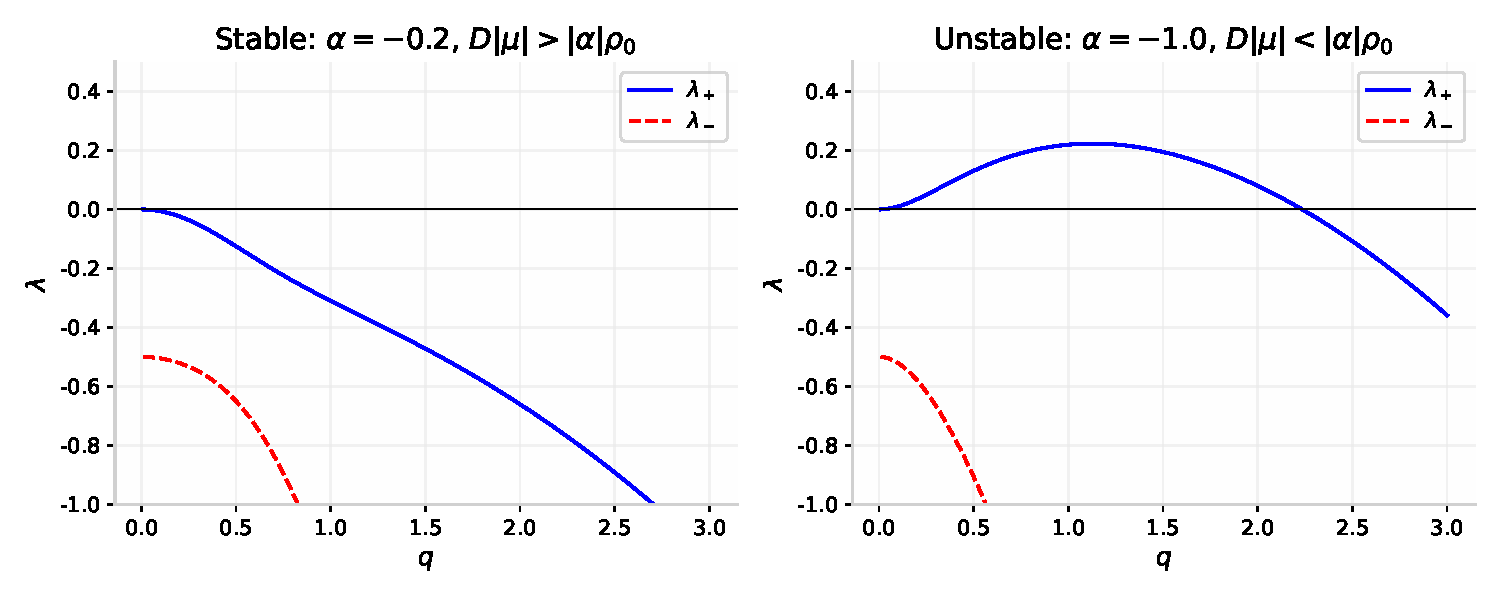
\includegraphics[width=0.85\textwidth]{figs/dispersion_relation.pdf} 
    \caption{Dispersion relation $\lambda(q)$ for the continuum chemotaxis model with $D=1$, $D_c=0.1$, $\mu=-0.5$, $\rho_0=1$.  \textbf{Left:} stable regime ($\alpha=-0.2$, $D|\mu|>|\alpha|\rho_0$); both eigenvalues are negative for all $q$.  \textbf{Right:} unstable regime ($\alpha=-1.0$, $D|\mu|<|\alpha|\rho_0$); the slow density mode $\lambda_{+}$ becomes positive at long wavelengths, signalling a linear instability of the homogeneous state.}
    \label{fig:dispersion}
\end{figure}

\paragraph{Physical interpretation.}
The long-wave instability in the chemorepulsive--consumption regime has a simple physical interpretation.  A local excess of particles consumes more chemical ($-\rho$), creating a local depression in $c$.  Because the particles are chemorepulsive ($\alpha<0$), they drift toward lower concentrations, i.e. toward the very region that already has an excess of particles.  This constitutes a positive feedback loop: density fluctuations seed chemical depressions, which in turn attract more particles and amplify the original fluctuation.  Diffusion competes against this feedback; the instability threshold \eqref{eq:chemorepulsion_stability} states that the effect wins when the chemotactic drift $|\alpha|\rho_0$ exceeds the diffusive damping $D|\mu|$ set by particle diffusion and chemical decay.  Notably, because the instability is strongest at $q\to 0$, the resulting clustering is large-scale and long-ranged, a feature that will be important when discussing the hyperuniform character of the density field.



\end{document}